\chapter{Design and Solution}
\section{Gathering Data}
% TODO: Thu thập dữ liệu và phân loại như thế nào -> Lấy từ web ..., các video thủ ngữ trên zootube
% TODO: Tiến hành tổng hợp và phân loại -> tổng hợp thành bảng, phần loại từ thành các pattern, location, direction để chuẩn bị cho mấy mục dưới
% TODO: Chèn hình về cái sheet vào



Before designing a system that can translate sign language, we must know what makes a word in sign language and where to collect the data. After a moment of observing the sign language on the website \url{https://tudienngonngukyhieu.com/}, we found an interesting point that some of the words tend to have the same pattern. Moreover, the sign's meaning depends on the direction and location that the sign has. And some of the terms need movements of the hands or fingers to represent the meaning. Hence, we can somehow convert a word from sign language into Vietnamese with those four factors.

But first, we need to collect the sign language data for the model training phase in this thesis. Fortunately, the site https://tudienngonngukyhieu.com/ is considered the library with enough words in sign language that we need. Moreover, we learned some of the words from videos on youtube, taught by Mrs. Le Thi Thu Xuong, and channel CDS, a center for the Deaf in central Vietnam. Hence, we can train and test our system on our own.

To preparing data, we collect many word from the website and youtube channel. Then, we label and seperate it into many element which we will discuss later in section about hand state (\ref{sec:handstate}). We made the google sheet for the data we gathered. In this file, we have prepare many word were labeled (see figure \ref{fig:Chap4-Label-Word}). Beside, we have a sheet for many hand shape (see in figure \ref{fig:Chap4-Sheet-Pattern}) which help us to classifying hand pattern.


\begin{figure}[H]
	\centering
	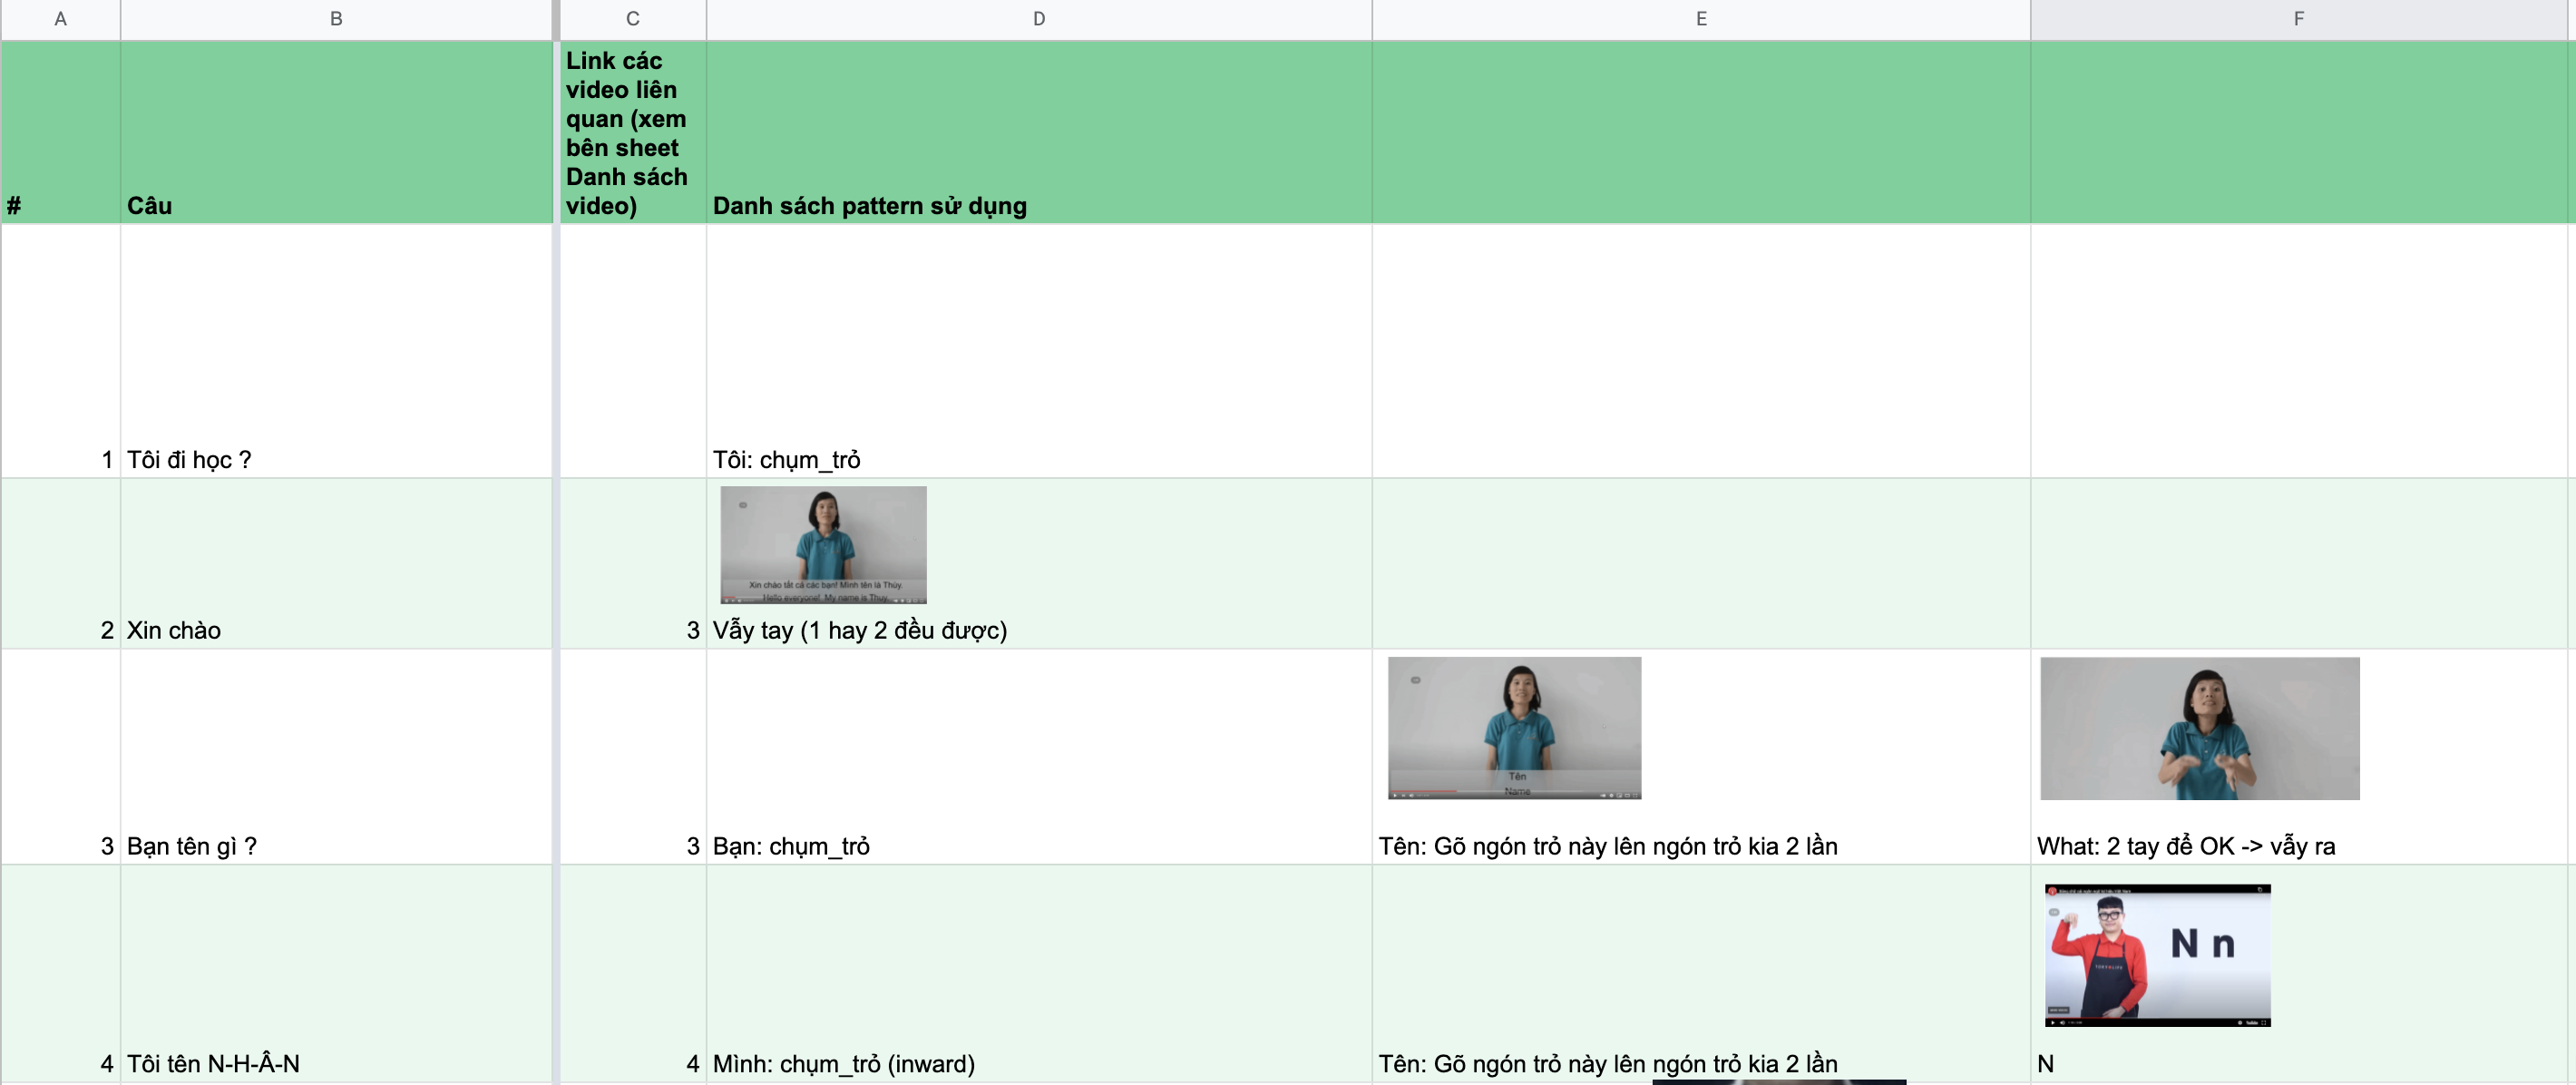
\includegraphics[width=0.9\textwidth]{img/Chap4/Label-Word.png}
	\caption{Google sheet about word labeled}
	\label{fig:Chap4-Label-Word}
\end{figure}

\begin{figure}[H]
	\centering
	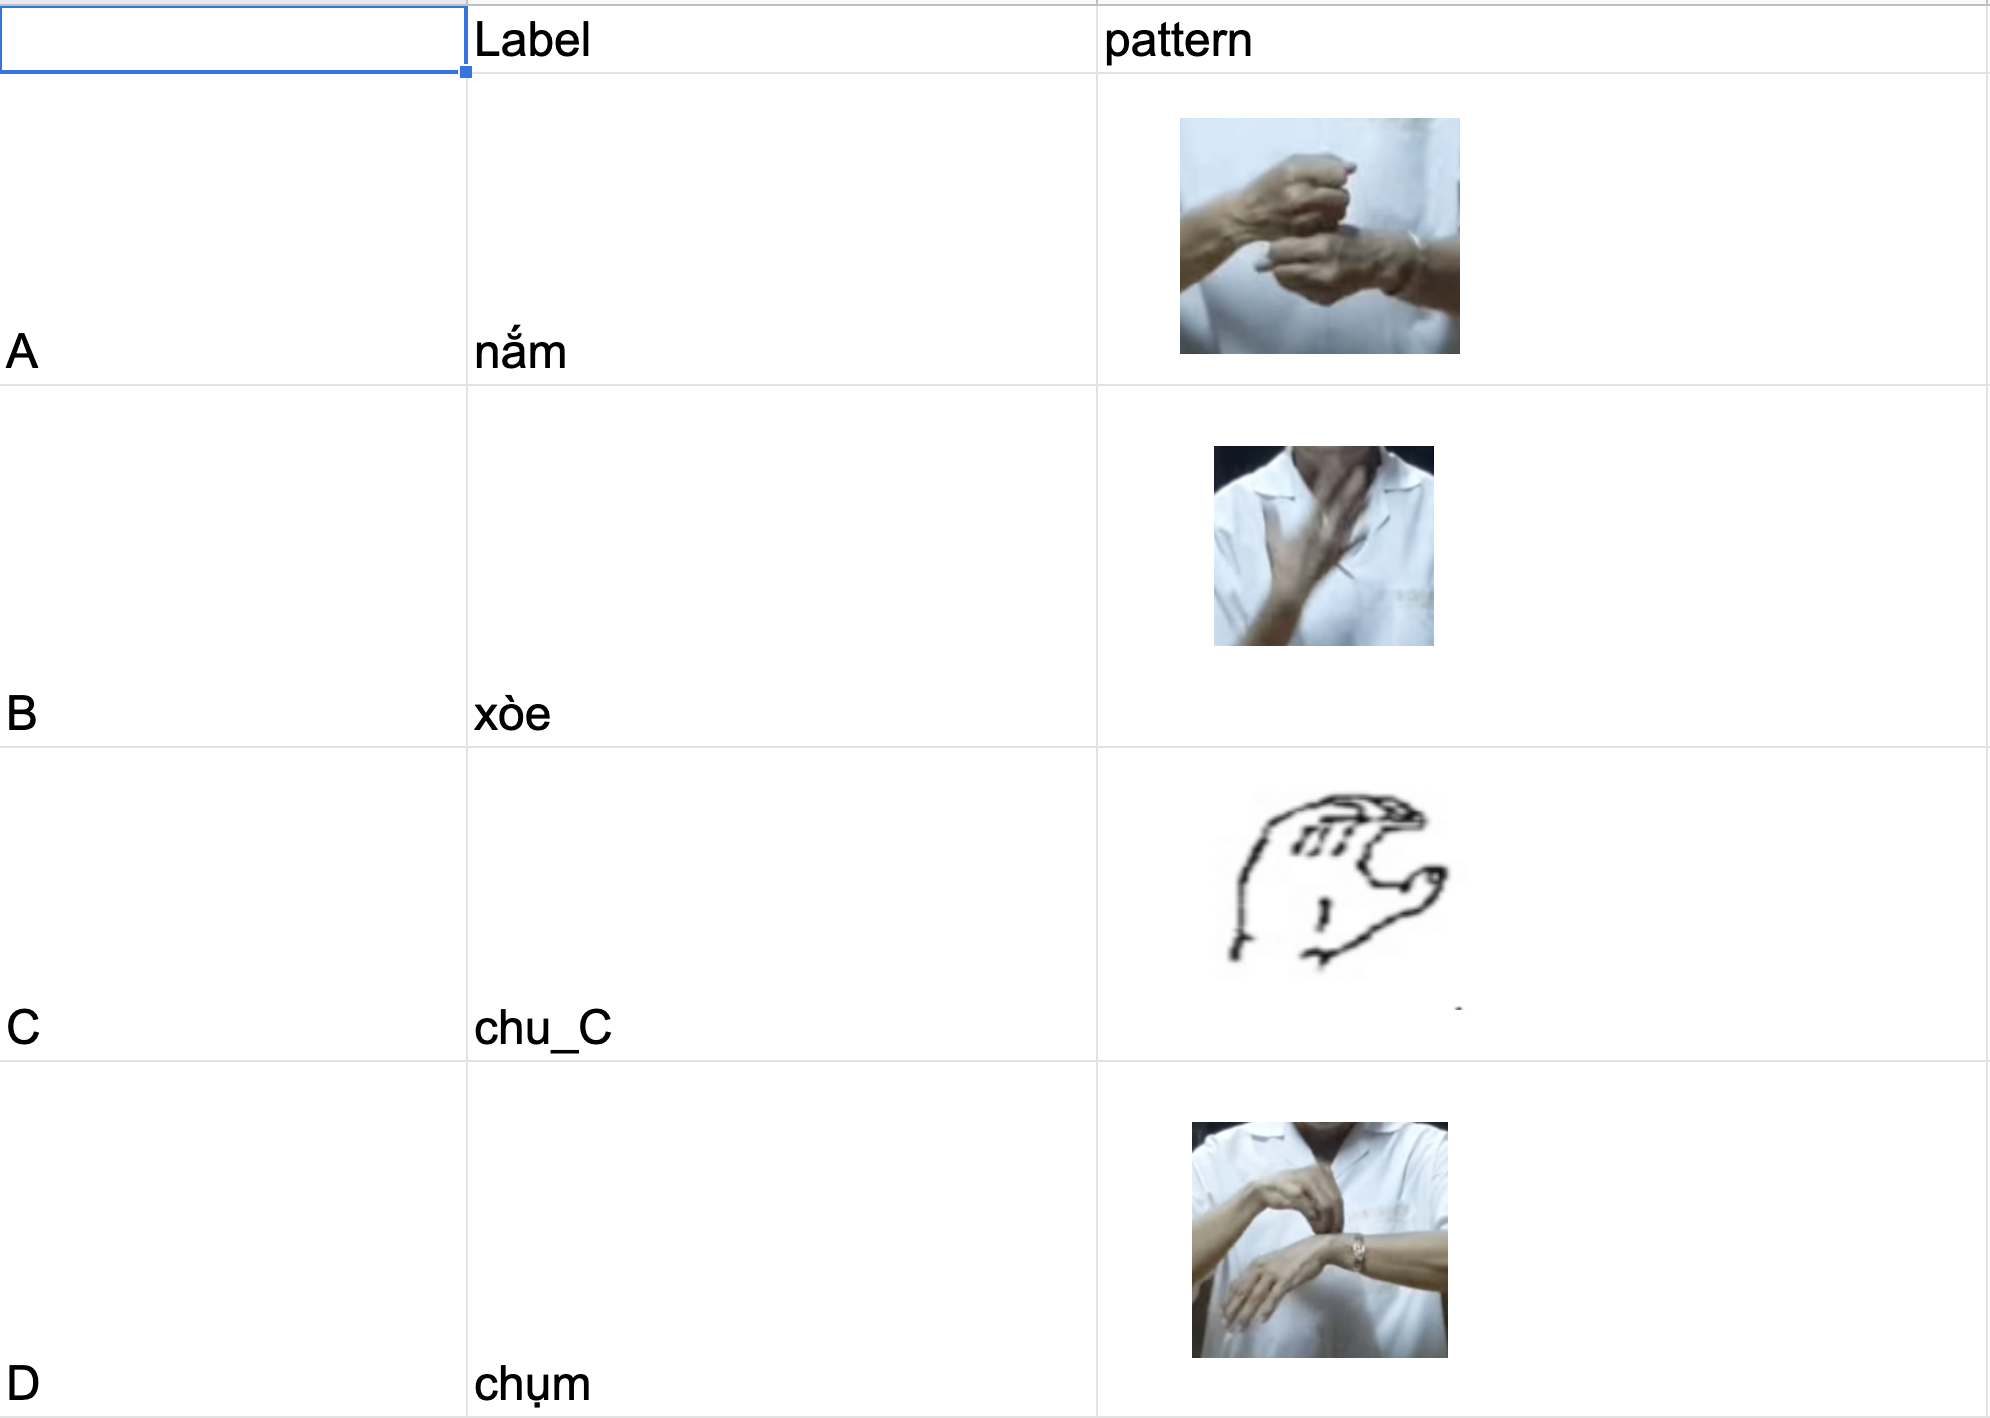
\includegraphics[width=0.9\textwidth]{img/Chap4/Sheet-Pattern.png}
	\caption{Google sheet about Hand Shape can be recognized}
	\label{fig:Chap4-Sheet-Pattern}
\end{figure}



\section{System Structure}

Overall, the system includes three parts of hardware modules: a camera module, the user's smartphone, and the server. Among those modules, the crucial one that handles the most complicated work is the server, which we will focus on in this thesis.

Our sign language translating artificial intelligence system includes six main modules: hand pattern recognition, direction determination, location detection, action detection, word decoder, and text to speech (figure \ref{fig:Chap4-OverviewOfTheSystemModules-Old}). Firstly, the system continuously captures the hand's motion, processes it with the hand landmark model, and then puts it into those modules. Each of them has a unique role, and after combining the first four modules' results (hand pattern, direction, location, and action detection), the word decoder module will take the output data and bring out the corresponding outcome. Then, the result will show up on the main screen; meanwhile, the phone will speak out that word.

\begin{figure}[H]
	\centering
	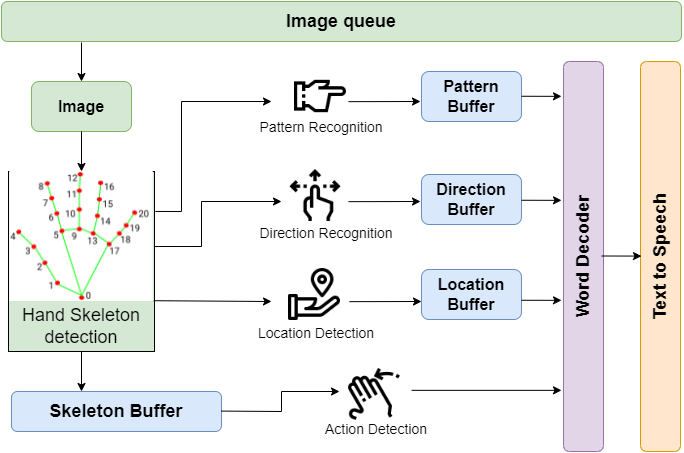
\includegraphics[width=0.9\textwidth]{img/Chap4/OverviewOfTheSystemModules-Old.png}
	\caption{Overview of the old system structure}
	\label{fig:Chap4-OverviewOfTheSystemModules-Old}
\end{figure}

Those six main modules mentioned above are the ones we planned up at the beginning of this thesis. However, during the implementing period, we found it hard to build the action detection module, despite going through most of the modules. It is problematic due to its demands on the smartphone and server.

There are words in sign language that contain many continuously moving patterns. There are a few solutions to detect which action the hands are doing; the first way is sending the whole video the camera captured to the server to process. This way, however, requires a strong connection between the camera module, smartphone, and the server and puts stress on the physical devices (the camera and smartphone); as a result, those devices will get hot quickly and can be damaged somehow. Another way is to increase the frame rate to get the action, but this one can also stress those devices; Moreover, we must have an algorithm continuously processing and detecting the movements, which, we admit, is hard to achieve.

Therefore, we had to deprecate that module and change our method to get the correct Vietnamese word to resolve that problem. Instead of using a combination of the four modules, including the action detection module, it now only has three left: pattern, direction, and location. Furthermore, in the word decoder module, we apply a heuristic search algorithm known as beam search, which uses the result of the three modules to look up the word in the database and return it to us. We will discuss each module's role and how it works in section \ref{sec:DetailImplementation}.

\begin{figure}[H]
	\centering
	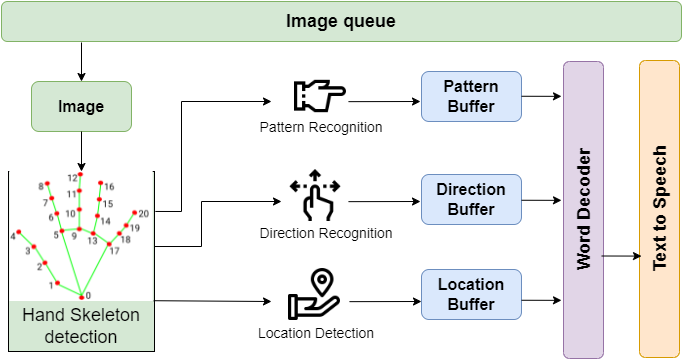
\includegraphics[width=0.9\textwidth]{img/Chap4/OverviewOfTheSystemModules-New.png}
	\caption{Overview of the new system structure}
	\label{fig:Chap4-OverviewOfTheSystemModules-New}
\end{figure}

\section{Detail Implementation}\label{sec:DetailImplementation}

\subsection{Hand pattern recognition}

Hand pattern recognition is the first and basic module of this system. While a person with disabilities does signs of sign language, his hands perform a series of different movements, where their hand may be spread out, clenched, or his fingers pointing out at something. Therefore, the role of this module is to recognize the pattern of the hands. Then combining the outcome with other modules, the system can give out the final result.

This module uses the output of the hand landmark model, which is a matrix size of 21. After calculating all the values in that matrix, we get a new matrix representing the distance between those 21 coordinates. Using the distance matrix as the input of CNN with the designed structure (see figure \ref{fig:Chap4-StructureOfConvolutionalNeuralNetwork}), as seen in figure \ref{fig:Chap4-OverviewOfTheSystemModules-New}, will tell us the pattern of the hand at the moment it is captured.

\begin{figure}[H]
	\centering
	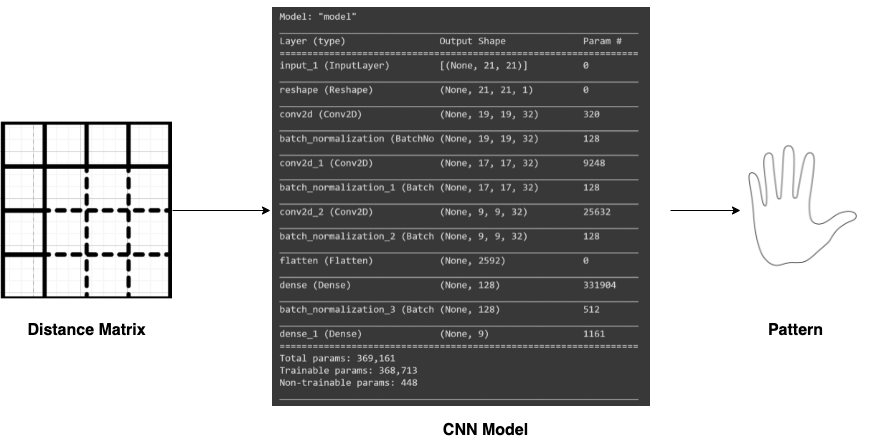
\includegraphics[width=\textwidth]{img/Chap4/Hand-Pattern-Reg-Model.png}
	\caption{Hand Pattern Recognition Pipe Line}
	\label{fig:Chap4-StructureOfConvolutionalNeuralNetwork}
\end{figure}

\subsection{Direction determination}

The directions of the hand include four directions, i.e., right, left, up, down, front, and back. Each hand's pattern combined with different directions leads to a different meaning. For example, the pattern that points at someone means the word "you"; on the other hand, when we point at ourselves, it means the word I (see figure \ref{fig:Chap4-WordYouInSignLanguage} and figure \ref{fig:Chap4-WordIInSignLanguage}).

\begin{figure}[H]
	\centering
	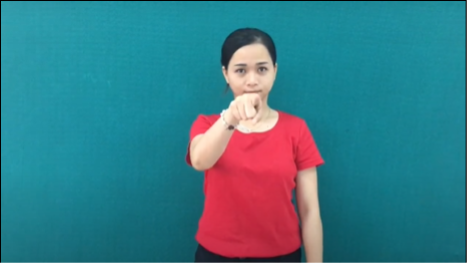
\includegraphics[width=0.6\textwidth]{img/Chap4/WordYouInSignLanguage.png}
	\caption{Word "You" (bạn) in sign language}
	\label{fig:Chap4-WordYouInSignLanguage}
\end{figure}

\begin{figure}[H]
	\centering
	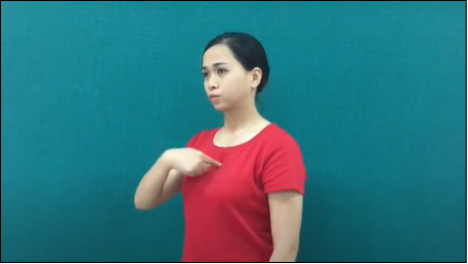
\includegraphics[width=0.6\textwidth]{img/Chap4/WordIInSignLanguage.png}
	\caption{Word "I" (tôi) in sign language}
	\label{fig:Chap4-WordIInSignLanguage}
\end{figure}

To determine the hand's direction, we use the hand landmark model provided in MediaPipe (see section \ref{sec:MediaPipe}). The inception here is that we calculate the distance between the tip of the index finger and the wrist, which can be called \textbf{vector(0, 8)}, then project it to the axis Ox, Oy, Oz, respectively. After that, we take each of those coordinates and compare them with the others. Finally, the one with the immense value will tell which axis the hand is on; besides, with the direction from the wrist to the tip of the index finger projected on that corresponding axis, we will know which direction the hand is.

\begin{figure}[H]
	\centering
	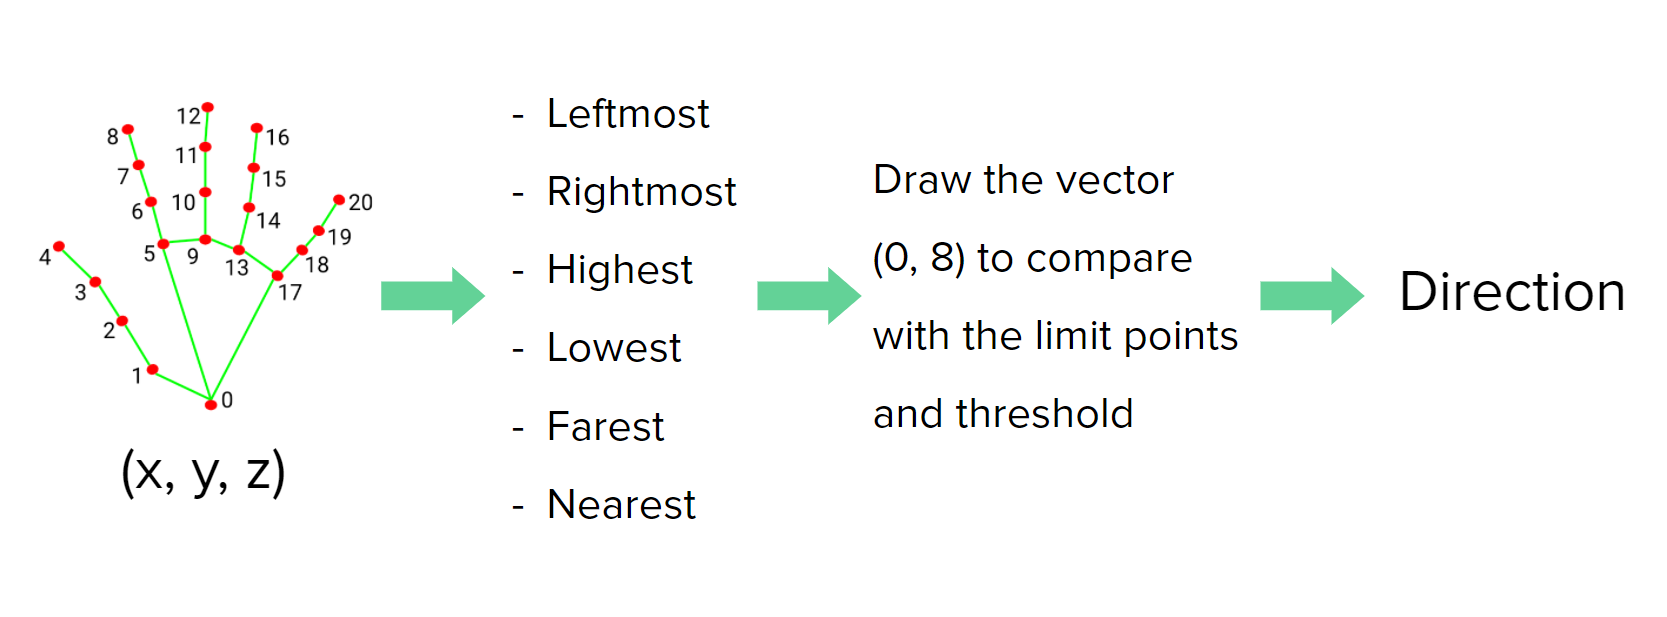
\includegraphics[width=\textwidth]{img/Chap4/DirectionSteps.png}
	\caption{Steps to detect the direction of the hand}
	\label{fig:Chap4-DirectionSteps}
\end{figure}

For instance, a hand is known to be pointing toward the left direction. The value of the distance, when projected on the axis Ox, will be the biggest one among the three projected values. Then, calculate the vector drawn from the wrist to the tip of the index finger; we will know the direction of the hand itself.

\begin{figure}[H]
	\centering
	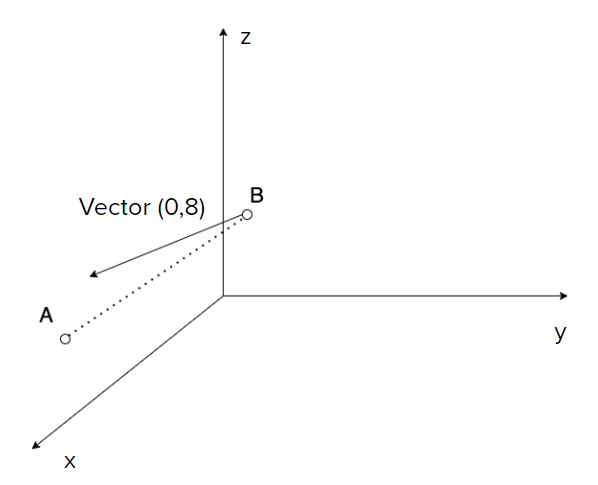
\includegraphics[width=0.6\textwidth]{img/Chap4/vector0-8-forwardLeft.png}
	\caption{Vector(0, 8) represent the hand pointing toward the left}
	\label{fig:Chap4-vector0-8-forwardLeft}
\end{figure}

\subsection{Location detection}

Locations of hand vary, is the hand put at forehead, mouth or the chest level, and so on. Every hand pattern that goes with every location will result in different words. Nevertheless, it is hard for the AI to know the hand's coordinates with only one camera, and its view is from above (see figure \ref{fig:Chap4-ViewFromCamera}). However, we came up with some solutions to this issue.

The zooming method is the first approach we use to detect the hand location. In this solution, we will take images of the hand and calculate the size of the hand in every frame in order to know whether that hand is getting larger or smaller. Hence, if that hand is smaller than before, it means the hand is getting far away from the camera, and its location is somewhere at the chest level or the stomach level. Otherwise, the hand's location is nearer to the camera, at the mouth, nose, or forehead level.

\begin{figure}[H]
	\centering
	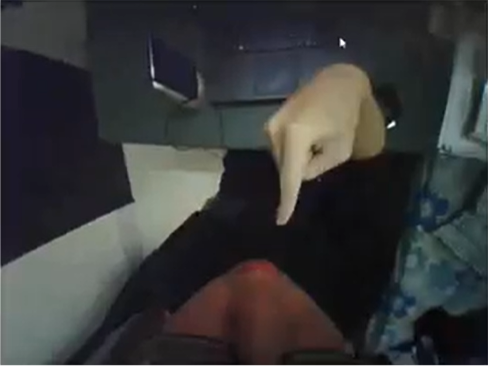
\includegraphics[width=0.6\textwidth]{img/Chap4/ViewFromCamera.png}
	\caption{View from the camera module}
	\label{fig:Chap4-ViewFromCamera}
\end{figure}

Nonetheless, the above solution still has an issue: every man's hand has a different size, and the system does not know the correct position of the hand. Therefore, another solution is to use a wide-angle camera and set it away from the forehead. With this solution, the camera can have a much broader view. Yet, since we only have a normal-angle camera, we could not try out this solution and confirm its suitability.

Another solution to detect the hand's location is using an ultrasonic sensor. In short, this sensor is an instrument that measures the distance to an object using ultrasonic sound waves (see figure \ref{fig:Chap4-UltrasonicSensorFunction}). It works by emitting a sound wave with a frequency above the human hearing range. The sensor's transducer functions as a microphone, receiving and transmitting ultrasonic sound. The sensor measures the time between sending and receiving an ultrasonic pulse to determine the distance to a target.

\begin{figure}[H]
	\centering
	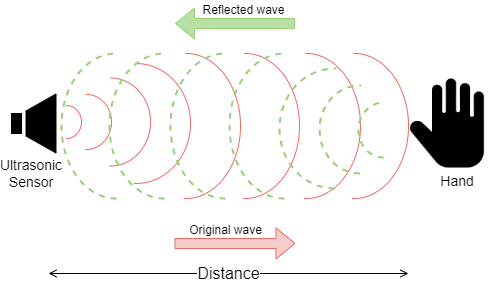
\includegraphics[width=0.7\textwidth]{img/Chap4/UltrasonicSensorFunction.png}
	\caption{Illustration of how the ultrasonic sensor works}
	\label{fig:Chap4-UltrasonicSensorFunction}
\end{figure}

\begin{wrapfigure}{r}{0.475\textwidth}
  \begin{center}
  	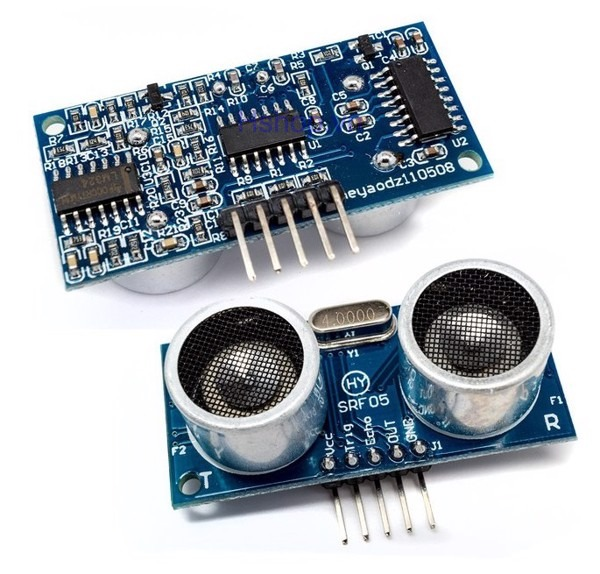
\includegraphics[width=0.3\textwidth]{img/Chap4/UltrasonicSensor.jpeg}
  \end{center}
	\caption{The ultrasonic sensor HY-SRF05}
  \label{fig:Chap4-UltrasonicSensorHYSRF05}
\end{wrapfigure}

In the thesis, the one we use for this module is the ultrasonic sensor HY-SRF05 (figure \ref{fig:Chap4-UltrasonicSensorHYSRF05}), which is relatively cheap and meets our demand in measuring the distance between the camera and the hand. According to the retailer, the wide-angle this sensor can scan is up to 15 degrees. Moreover, its scanning range is between 2 cm and 450 cm, with the relative error fluctuating around 0.3 cm. Besides, the most accurate measurement distance is under 100 cm, which is more than enough when it comes to measuring from the forehead to the user's waist.

However, the sensor method has not yet achieved the desired effect. The reason is that the sensor can only detect one hand at a time, but what if sign language using 2 hands at the same time, using only the sensor will not bring feasible results.

From there, we offer another solution for measuring this distance as follows. Replace that method of distance by sensor with a distance measurement method based on object size. It is almost similar to the zooming method, but this method is better in that it will not depend on the size of the hand, so it is perfectly suitable for determining the distance for the problem we are trying to solve.

This method is as follows. We will use the following formula:
\begin{center}
  $ distance\_predict = A*distance\_input + B*distance\_input + C $ 
\end{center}

In which, $distance\_input$ will be the distance between two points (5,17) on the hand model taken from the MediaPipe model and $distance\_predict$ will be the distance from the camera to the hand. \\

The trio of coefficients A, B, C will be determined by interpolating the above polynomial with a pre-prepared data set. After having the above three coefficients, combined with calculating the distance between 2 points 5 and 17, we will easily deduce the distance of the hand.



Consequently, after getting the result from this location module, we put it within a hand state. And we will discuss how that hand state will help us translate sign language into Vietnamese in the following section.

% TODO
  % New approach : Sử dựng phương pháp khác để có thể đo khoảng cách
  % [ ] Thêm hình ảnh 
  % [ ] Giải thích
  
  % Thay thế phương pháp đo khoảng cách bằng sóng âm bằng phương pháp đo khoảng cách dựa trên hình ảnh 
  % Công thức: ...
  % Sử dụng phép nội suy đa thức để suy ra giá trị của các tham số A,B,C. 
  
  % Chúng ta sẽ tính khoảng cách giữa 2 điểm 5 và 17 trên bàn tay, sau đó sử dụng kết quả vừa tính toán được và công thức đã nêu ở trên để suy ra khoảng cách thực tế của bàn tay

  % Sau khi khoảng cách đã được ước lượng, ta sẽ suy ra được vị trí hiện tại của bàn tay đang ở đâu trên cơ thể (đầu, ngực hay bụng)
  





\subsection{Word decoder}
% TODO:   Previous approach 

% [x] How to map word ?

% TODO:   New approach

% [x] Punish function

% [x] Using beam search

% [x] CTC decode

% [x] Flow

% [x] Expected result

% [...] Difficult and proposed solution

% [...] Dịch sang tiếng anh

% [...] Thêm các hình ảnh


% TODO: With previous approach

As discussed above, there are considerable technical difficulties in implementing the action detection module. We did some research and proposed a new model to resolve these problems. As a result, this change affects the word decoder module, which needs some adjustments.

The previous model decodes a word into four factors: pattern, location, direction, and action. After getting the outputs from the four modules, it will search the database to find the corresponding word. figure \ref{fig:Chap4-MapWord} illustrates how an input containing four factors is mapped to the correct word in the database. Applying a basic searching algorithm, we have the system find the most appropriate word. If it can not find any, it will replace or deprecate some parts of the input and try again to find another word. After decoding and finding the suitable word, the application will display that word on the screen.

\begin{figure}[H]
	\centering
	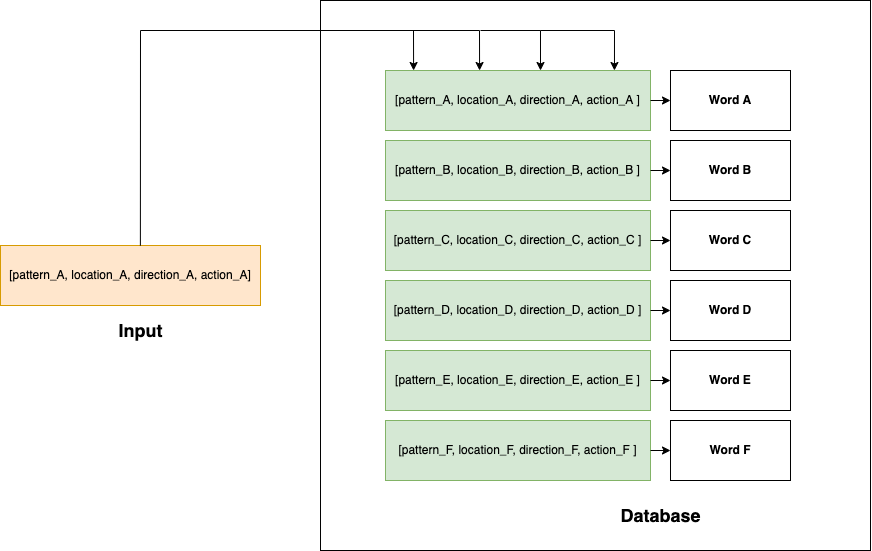
\includegraphics[width=\textwidth]{img/Chap4/MapWord.png}
	\caption{Map one to one data from four component with word in database and get result}
	\label{fig:Chap4-MapWord}
\end{figure}

\subsubsection{ Introduction to handstate }\label{sec:handstate}

Right after the deprecation of the action detection module, the question that comes up is how we can find the correct word without that module. Therefore, we propose a different model for a word that is not decoded into four factors like the previous model. It only contains three elements left: pattern, direction, and location. Consequently, each set of those three elements is called a hand state (\ref{fig:Chap4-HandState}), and a word is decoded into many different hand states.

This concept of hand state comes from the research of natural language processing, in which a word is composed of many characters. Accordingly, a word is concatenated from many hand states in this thesis. Then, we will get the desired word when going through the processing steps that we will discuss later in this proposal.

\begin{figure}[H]
  \centering
  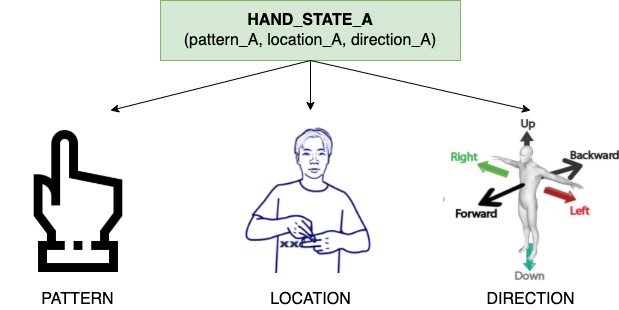
\includegraphics[width=0.6\textwidth]{img/Chap4/HandState.png}
  \caption{ Hand State which construct from pattern, location and direction}
  \label{fig:Chap4-HandState}
\end{figure}

\subsubsection{ Using beam search and CTC decode to map word}

After we have grasped the concept of hand state, we will come to the essential part of the model: converting the received hand states into words.
      
\begin{figure}[H]
  \centering
  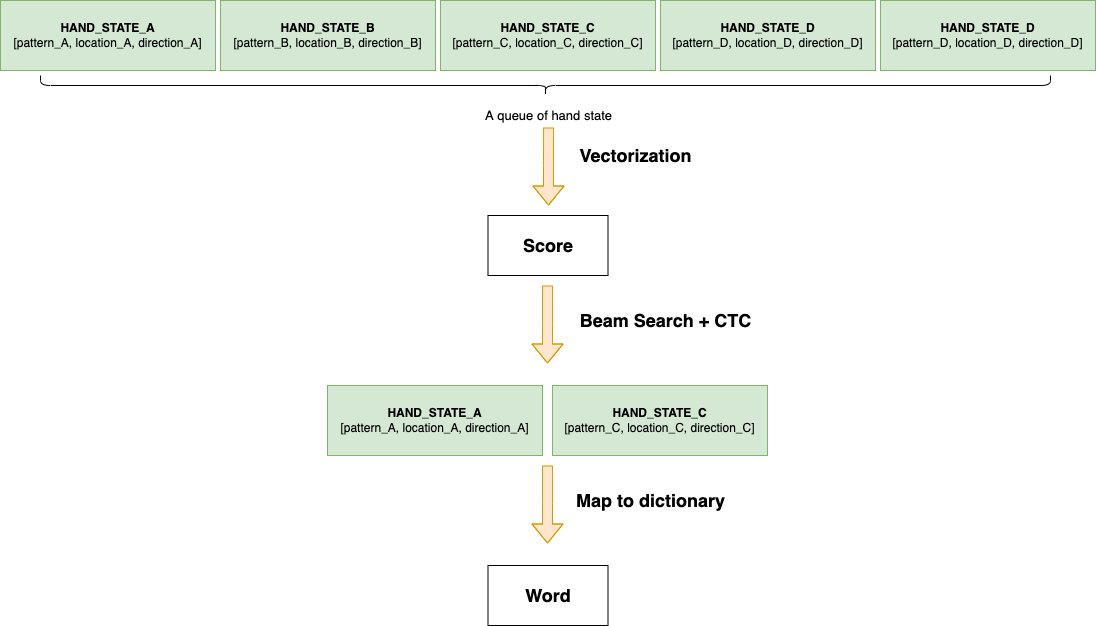
\includegraphics[width=\textwidth]{img/Chap4/Architechture.png}
  \caption{Architecture}
  \label{fig:Chap4-Architechture}
\end{figure}

Figure \ref{fig:Chap4-Architechture} is the model proposed by the authors for this section. The input will be a queue of hand states taken from the previous three components. Here, in our conventions, the queue length is set to 5, but it is not the final number, as we need more calculations and experimentation to find the right queue length. This model consists of three steps:

\begin{enumerate}
  \item \textbf{Vectorization:} This step converts a queue of many hand states \ref{fig:Chap4-HandStateQueue} into a matrix as input for beam search.
  \item \textbf{Beam search:} In this step, we will perform a beam search algorithm to choose which hand states are suitable for the input from the database. Besides, we propose using the CTC decode model to eliminate the wrong hand states or previous duplicated hand states, increasing the model's efficiency.
  \item \textbf{Map to the dictionary:} And finally, after going through the above two steps, from the initial queue, we will get the most likely hand states. Our job is to map these hand states to the database and find the correct word.
\end{enumerate}
      
\subsubsection{ Vectorization }
% TODO: Why we need punish
% TODO: how to perform -> Trình bày cách đánh giá như thế nào, cách trừ điểm và các phương châm đánh giá
% TODO: Sau khi punish dùng hàm softmax để chuyển các giá trị về dạng xác suất

When we get to this step, we get a queue of hand states. Because before entering the beam search module, we need a matrix representing the correlation between the outputs received from the components and the data in the database.

\begin{figure}[H]
  \centering
  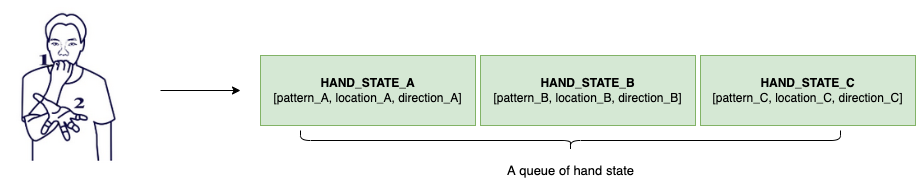
\includegraphics[width=\textwidth]{img/Chap4/HandStateQueue.png}
  \caption{A queue of hand state which get from three component in section ... }
  \label{fig:Chap4-HandStateQueue}
\end{figure}

From this queue, we will cycle through each hand state, compare it with the available hand state database, and evaluate the score for it based on the following principles \ref{fig:Chap4-Vectorization}:

\begin{enumerate}
  \item The score will be increased if the hand state matches the word in the database.
  \item Otherwise, the score will be decreased if that hand state does not match any.
\end{enumerate}

\begin{figure}[H]
  \centering
  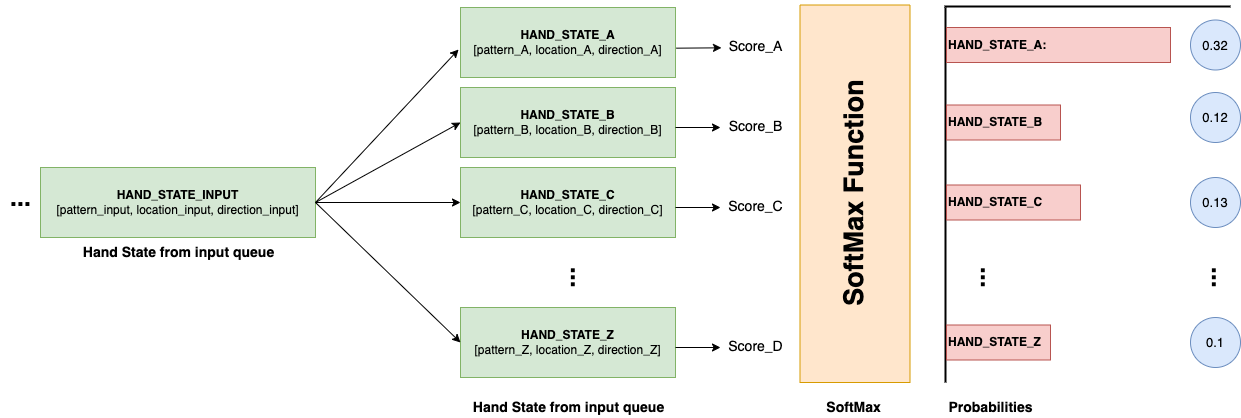
\includegraphics[width=\textwidth]{img/Chap4/Vectorization.png}
  \caption{ Vectorization }
  \label{fig:Chap4-Vectorization}
\end{figure}
% TODO: Change to Math
In the first principle, The more similarities the hand state retrieved from the queue has compared to that in the database, the higher it is scored. For example, in the database, we have a hand state as follows: 
$\begin{bmatrix}
  pattern \_ A & location \_ A & direction \_ A
\end{bmatrix}$
, and the hand state we get from the input is 
$\begin{bmatrix}
  pattern \_ A & location \_ A & direction \_ A
\end{bmatrix}$
then this hand state will be rated higher than the hand state 
$\begin{bmatrix}
  pattern \_ A & location \_ A & direction \_ B
\end{bmatrix}$
. And so on, we will, in turn, score the hand states taken from the queue.

On the second point, the minus point is evaluated based on its matching pattern with the hand states in the database. When the system recognizes patterns from the hand pattern recognition module (using the vision approach), it is likely to be wrong detected or mistaken. To resolve this problem and maximize the accuracy of the result, we put out a rule. With those patterns that are usually hard to detect, the minus point will be lower than simple ones. In short, the more complex the pattern to be recognized, the smaller the minus point is going to be.

% + Khi đánh giá các hand state, đối với trường hợp so trùng 2 pattern. Do các pattern này được nhận diện từ module hand pattern regconition (vision approach), do đó, sẽ có khả năng bị nhận diện bị sai, hoặc bị nhầm. Vì lẽ đó, để có thể đánh giá một cách chính xác và công bằng nhất có thể thì ở đây, đối với những pattern hay bị nhận diện sai, ta sẽ trừ điểm thấp và ngược lại, với những pattern đơn giản mà hệ thống lại nhận diện sai thì sẽ bị trừ điểm nhiều hơn.
      
After completing the above evaluation and scoring step, we will use a function to normalize the data (here, the authors use the softmax function \cite{SoftMax}) and return us a set of probabilities of the hand states in the row. Wait. We will use this set of probabilities as input for the beam search step.

\subsubsection{ Using beamsearch with CTC decode }
% TODO: Trình bày cách sử dụng beamsearch để tìm các cặp bộ 3
% TODO: Image beamsearch (get from ppt)
% TODO: Example
% TODO: Áp dụng CTC để handle một số trường hợp
% TODO: Các khó khăn gặp phải và hướng giải quyết

After passing the vectorization step, the hand states in our queue has been converted to a MxN matrix, where M is the length of the hand state's database and N is the length of queue.

By using beam search (\ref{fig:Chap4-BeamSearch}), we will get the most likely k hand state from the database. From the image below, we can imagine what happened later during beam search.

% Sau khi qua bước vectorizaion, các hand state trong hàng đợi của chúng ta
% đã được chuyển đổi thành một ma trận MxN với M là độ dài của cơ sở dữ liệu về
% các hand state và N là độ dài của hàng đợi.
      
% Bằng việc sử dụng beam search, từ sẽ thu được k hand state có khả năng nhất
% từ cơ sở dữ liệu. Từ hình ảnh bên dưới, ta có thể hình dung được những gì
% đã diễn ra sau trong quá trình thực hiện beam search

% FIXME: Insert image from ppt about matrix with beam search

\begin{figure}[H]
  \centering
  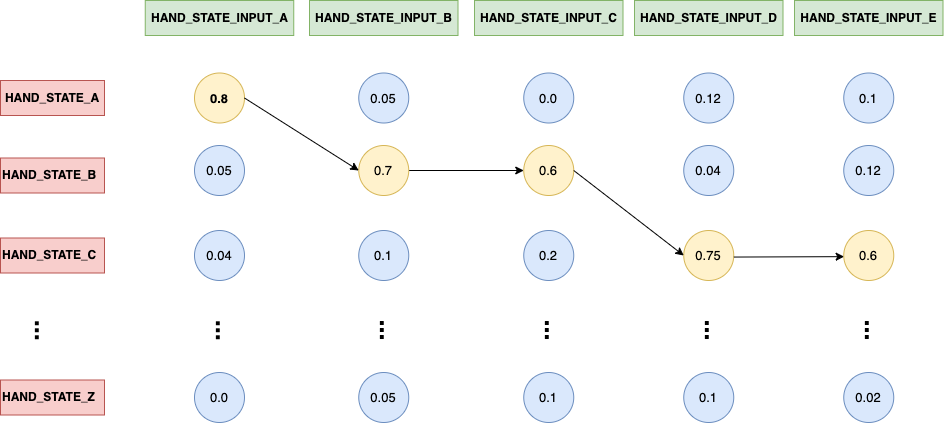
\includegraphics[width=\textwidth]{img/Chap4/BeamSearch.png}
  \caption{ Beam Search }
  \label{fig:Chap4-BeamSearch}
\end{figure}

However, as we can see that, after performing the beam search step, we will get a sequence of hand states whose length corresponds to the length of the input queue, these hand states can include duplicate hand states, or they can be wrong hand states. Therefore, we need to apply CTC algorithm to remove the hand states from infection. For the wrong hand states, in Vectorization step, we will set a threshold to discard these hand states and see it as a blank character. And after all step, after beam search CTC decode, we will get the desired result.

% Tuy nhiên, có thể thấy được rằng, sau khi thực hiện xong bước beamsearch,
% ta sẽ thu được một dãy các hand state có độ dài tương ứng với độ dài của hàng đợi
% , các hand state này có thể bao gồm những hand state bị trùng nhau, hoặc cũng có thể
% là những hand state bị sai. Do đó, ta cần áp dụng thêm CTC decode để loại bỏ các hand state
% bị trùng này. Đối với những hand state bị nhận sai từ những module trước thì ở bước Vectorization,
% ta sẽ đặt một threshold để loại bỏ những hand state này và xem như hand state đó là một ký tự rỗng (" ")
% và cuối cùng, sau khi áp dụng CTC decode vào, ta sẽ thu được kết quả mong muốn

% FIXME: Insert image about the result (get from ppt)

      
      
    \subsubsection{ Map to dictionary }
      % TODO: Cách map như thế nào

      \begin{figure}[H]
        \centering
        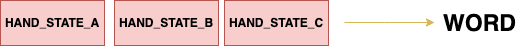
\includegraphics[width=\textwidth]{img/Chap4/Result.png}
        \caption{ Map to dictionary and get word }
        \label{fig:Chap4-Result}
      \end{figure}

      % Sau khi nhận được một tập các hand state có khả năng nhất, việc còn lại là
      % chúng ta sẽ map vào cơ sở dữ liệu, như cách mà chúng ta đã làm trong mục ..., 
      % nhưng thay vì map với bộ 4 thành phần thì ở đây, ta sẽ map với input các hand state thu được
      % từ bước ... .
      % Và như thế, ta sẽ thu được từ vựng mà không cần phải dùng tới module action detection.
      After getting a set of most likely hand states, all that remains is for us to map to the database, as we did in section above, but instaed of map with 4-component set, in here, we will map with input retrieved from this previous step. And finally, we will get the word (\ref{fig:Chap4-Result}) without using the action detect module.



\subsection{Text-to-speech}

In addition, sometimes, people do not always read the result from the phone's screen, so to make it easier for them to know the answer after translating process, the application can speak it out loud. Basically, one way to do this is to build a database of many sound files mapped with the corresponding word in Vietnamese. This approach, however, is not efficient as it requires a massive effort in creating the database. We must record every single word and map them all together.

Instead of using that approach, we use a well-known speech service from Google called Text-to-speech \cite{GG:Text-to-Speech}. According to Google, Text-to-Speech converts text input into natural human speech audio data. And this service supports many languages, including the one that we need, Vietnamese. With the provided API from that speech service, our application can speak up the result without an extensive sound database in the user's phone.

In fact, this API is a freemium service. Text-to-Speech costs are determined by the number of characters transmitted to the service each month to be synthesized into audio. Google states on their website that,  "The first 1 million characters for WaveNet voices are free each month. For Standard (non-WaveNet) voices, the first 4 million characters are free each month. After the free tier has been reached, Text-to-Speech is priced per 1 million text characters processed." This thesis only needs the standard (non-WaveNet) plan, which provides us 4 million characters free each month and only costs USD 4.00 per following 1 million characters. In the upcoming phases of building up the application, the number that we will use is negligible compared to 4 million free characters. Therefore, we decided to apply this Text-to-speech module using Google service in this thesis.





\subsection{The camera module}

After having discussed mainly the solutions and implementations of the soft modules in the system, we must move on to the main one that is considered to be the eyes of this thesis, which is the camera module. This section will discuss what parts are in a camera module and represent some images of a real one we built.

We can easily find the camera modules' parts from any retailer selling electrical components, robots, and Arduino kits. Additionally, in the current era of e-commerce, it is easier for us to find and compare those components that we need online. The parts required to build a camera module are listed below.

First, we need a camera part, and ESP32-CAM is the perfect one for this role. It is inexpensive and easy to use, making it ideal for our thesis that requires complex functions like image tracking and recognition. Furthermore, it integrates Wi-Fi, traditional Bluetooth, which help us in sending the images to the user's smartphone for the next steps in translating sign language.

Secondly, we need a converter adapter to help us sideload the program into the camera module. Besides, the third part that we need is the ultrasonic sensor mentioned in the TK section. It plays a role in location detection, which will tell the system the distance between hands and the camera module. Last but not least, this camera module needs a battery to power the whole module, and we reckon that the volume of about 100 mAh is fine.

Furthermore, there must be a box to store all the above parts. With the help of current 3D printing technology, we design that package on Tinkercad, an online 3D modeling program that runs on the web browser. After getting all the necessary components, we tried to put them all together and get the result below.

\begin{figure}[H]
	\centering
	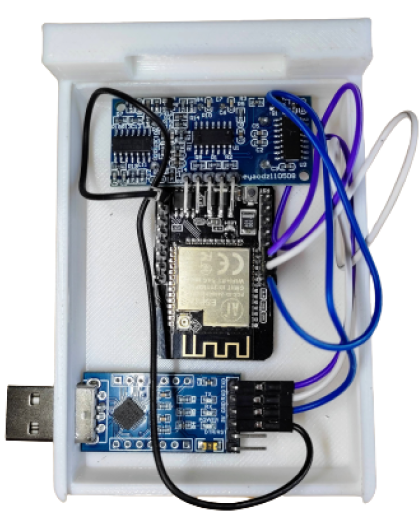
\includegraphics[width=0.45\textwidth]{img/Chap5/Prototype_View_inside.png}
	\caption{The components inside the camera module prototype}
\end{figure}

\begin{figure}[H]
	\centering
	\begin{subfigure}[b]{0.45\textwidth}
		\centering
		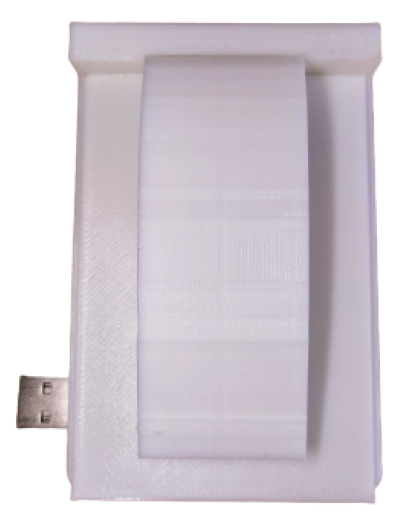
\includegraphics[width=\textwidth]{img/Chap5/Prototype_View_above.png}
	\end{subfigure}
	\hfill
	\begin{subfigure}[b]{0.46\textwidth}
		\centering
		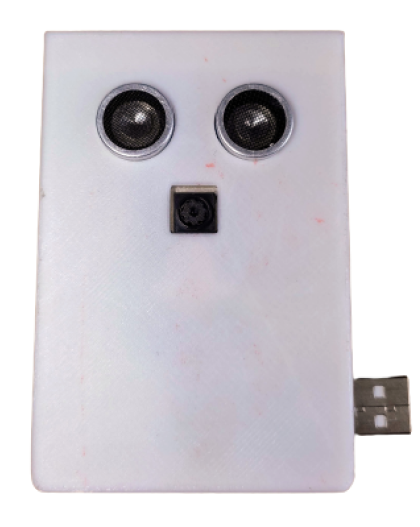
\includegraphics[width=\textwidth]{img/Chap5/Prototype_View_under.png}
	\end{subfigure}
	\caption{Views of the camera module prototype from the above and under}
\end{figure}

\begin{figure}[H]
	\centering
	\begin{subfigure}[b]{0.45\textwidth}
		\centering
		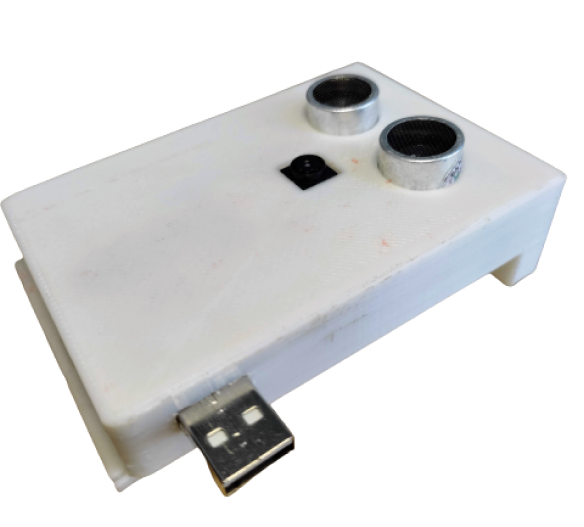
\includegraphics[width=\textwidth]{img/Chap5/Prototype_View_side_1.png}
	\end{subfigure}
	\hfill
	\begin{subfigure}[b]{0.45\textwidth}
		\centering
		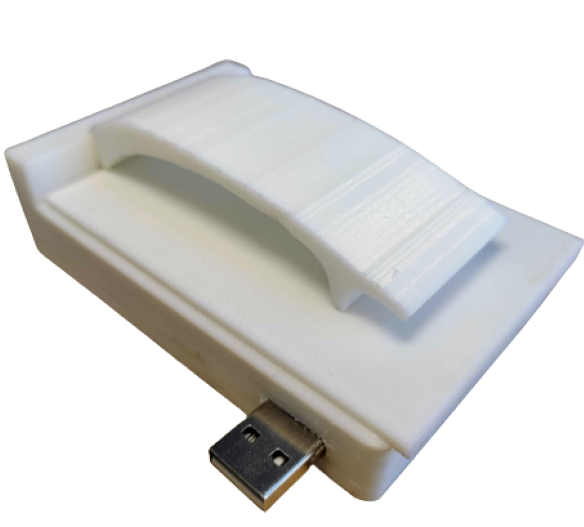
\includegraphics[width=\textwidth]{img/Chap5/Prototype_View_side_2.png}
	\end{subfigure}
	\caption{Views of the camera module prototype from the sides}
\end{figure}

Nevertheless, due to the smallest number that a 3D printer can print, the box's cover is a bit hard to put in. And the hanger that helped hang the box on the hat is not as flexible as we thought, so it needs a redesign.

\subsection{App design}

The application must satisfy user experience, and user interface demands. And during the research phase of this thesis, we did design a prototype for the application, including two more features besides the main one. Those features are a sign language dictionary and a learning system. We will talk more about those features in the later sections.

Before going through the design of this application, we must state that they do not cover all the screens needed for the application yet. And they are not the final design that we have. However, we have some conventions when designing this prototype, such as the corner is rounded and the colors are pale, not too bright, to make the users feel calm somehow and comfortable when using the application.

\begin{figure}[H]
	\centering
	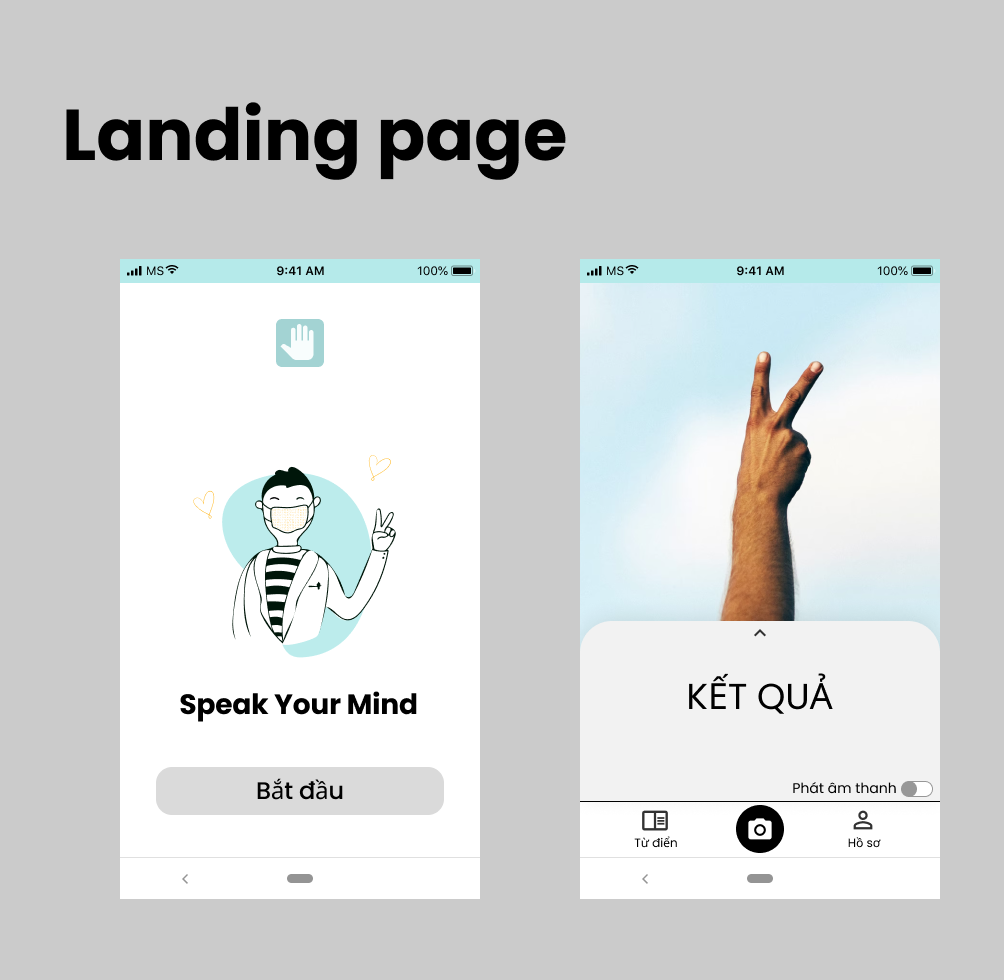
\includegraphics[width=0.8\textwidth]{img/Chap5/Landing_page.png}
	\caption{The landing page of the application}
\end{figure}

\begin{figure}[H]
	\centering
	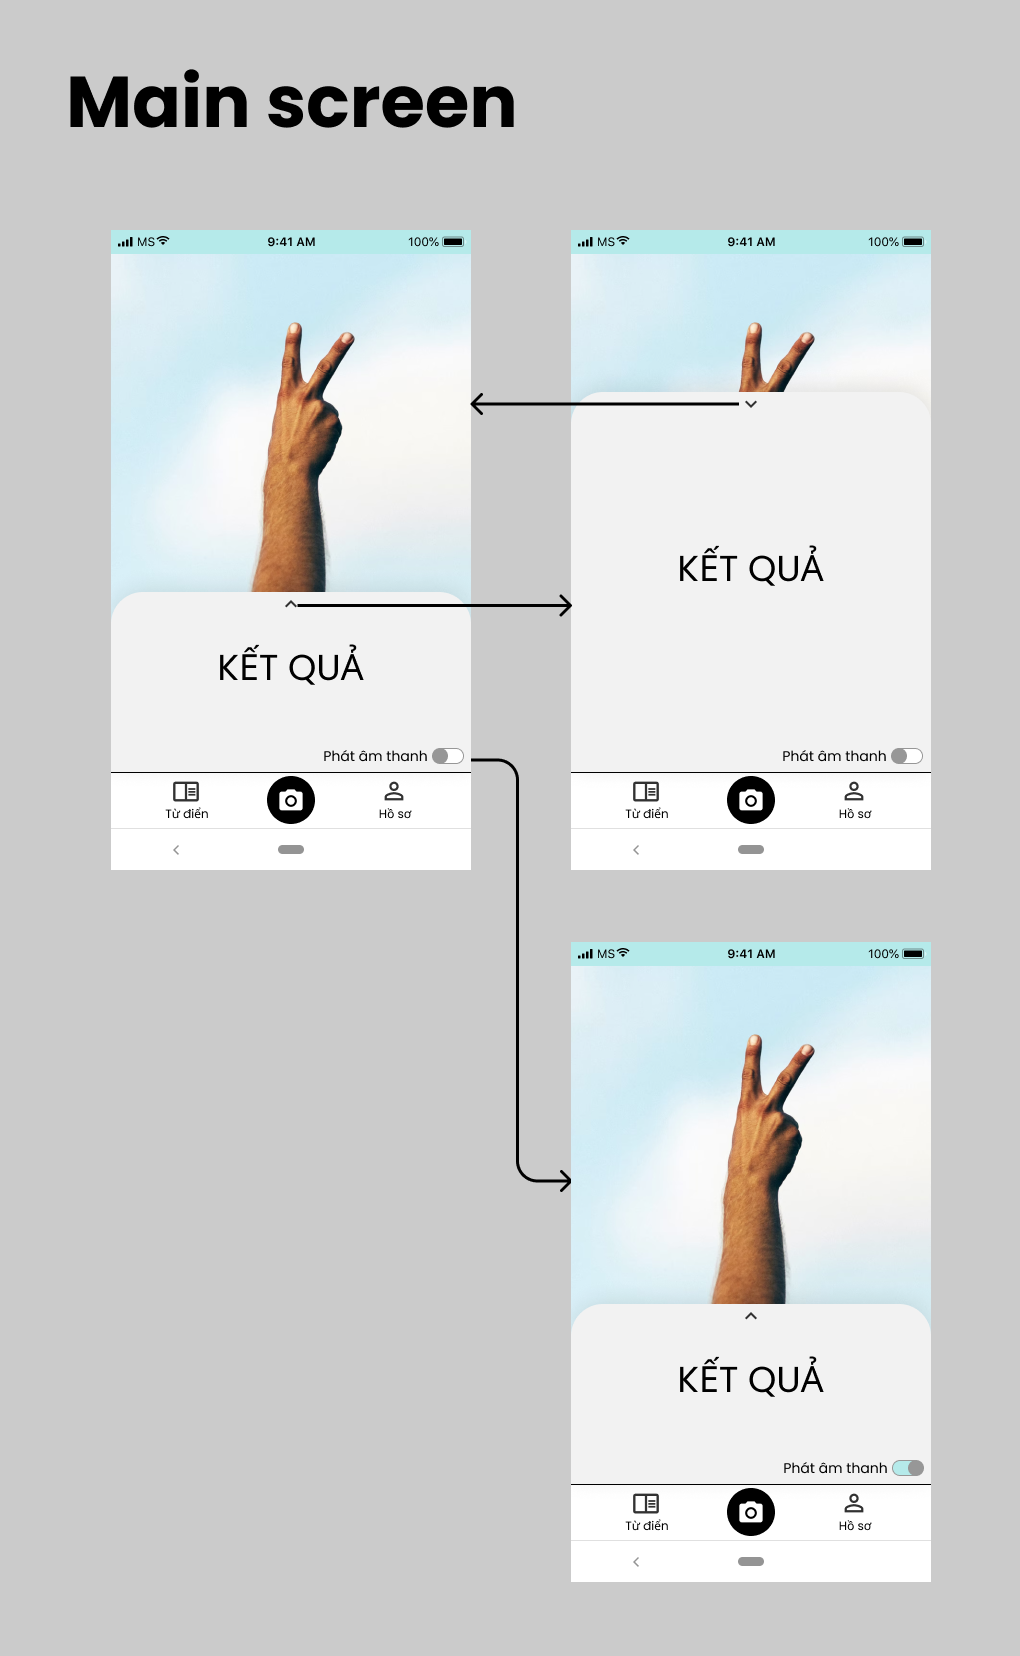
\includegraphics[height=0.8\textheight]{img/Chap5/Main_screen.png}
	\caption{The main screen of the application}
\end{figure}

\begin{figure}[H]
	\centering
	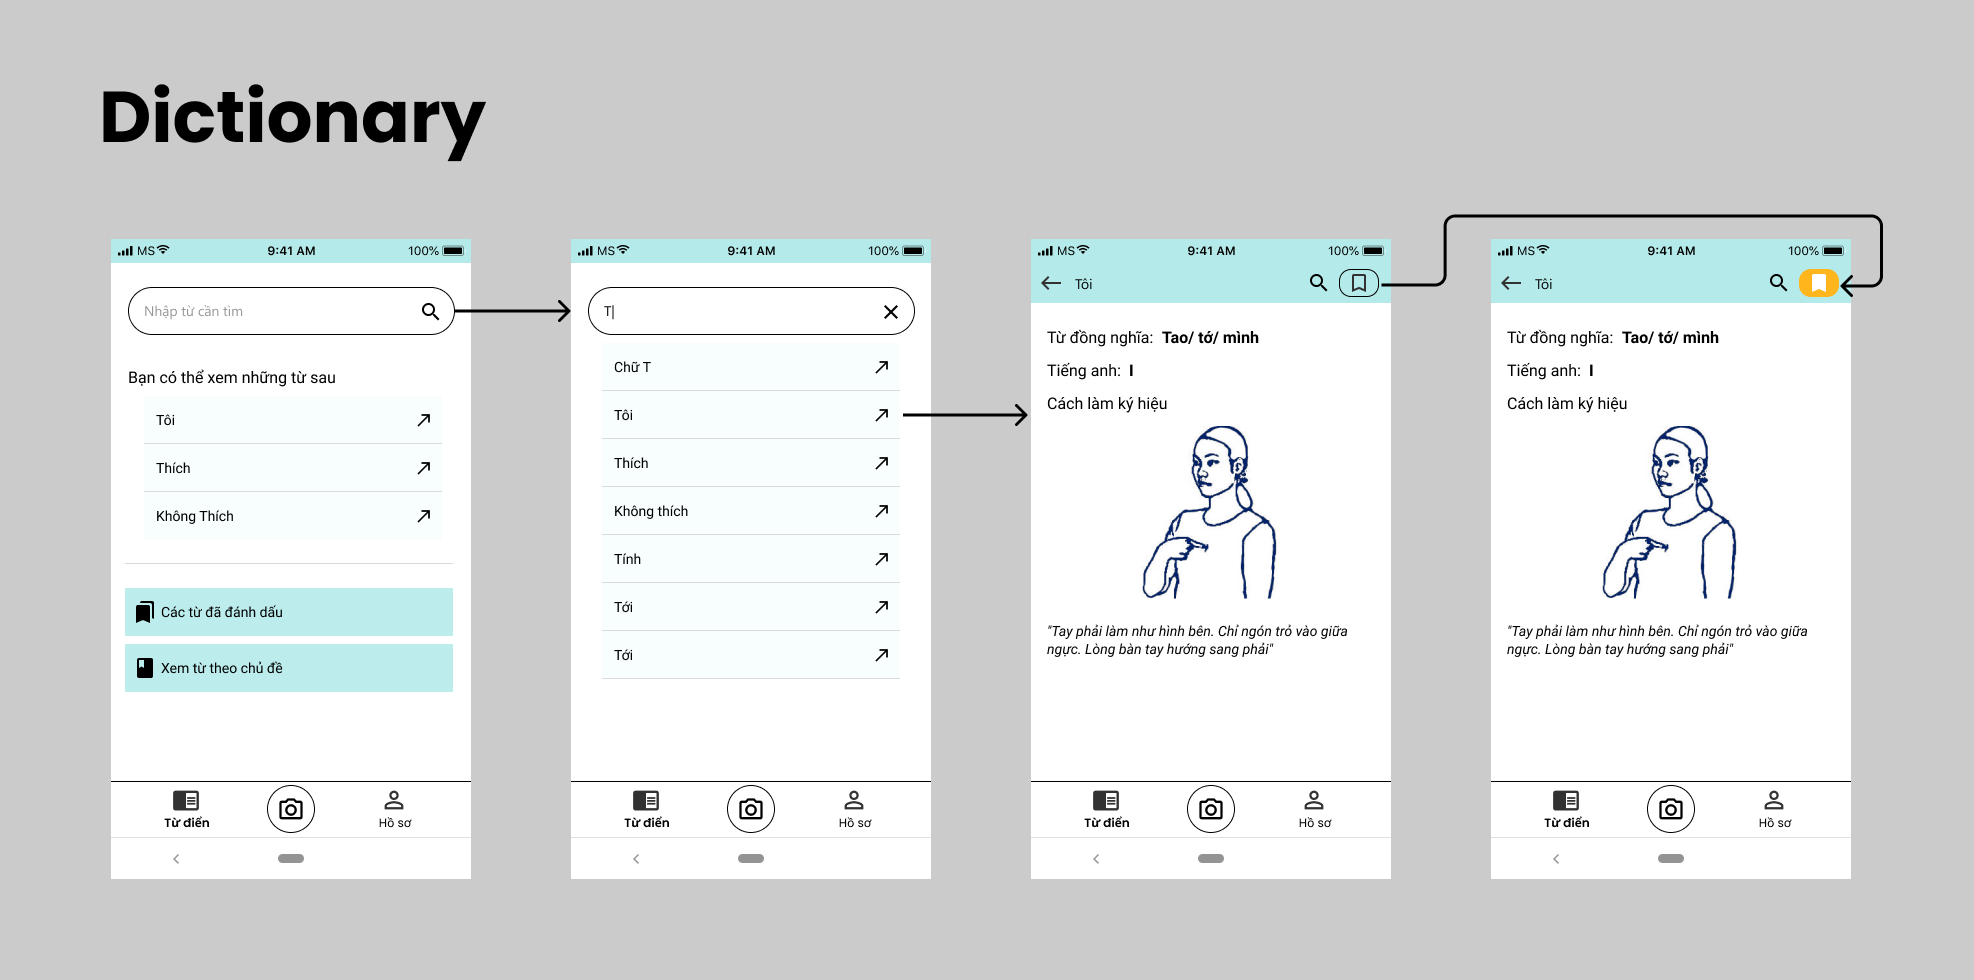
\includegraphics[width=\textwidth]{img/Chap5/Dictionary.png}
	\caption{The main screen of the application}
\end{figure}

\begin{figure}[H]
	\centering
	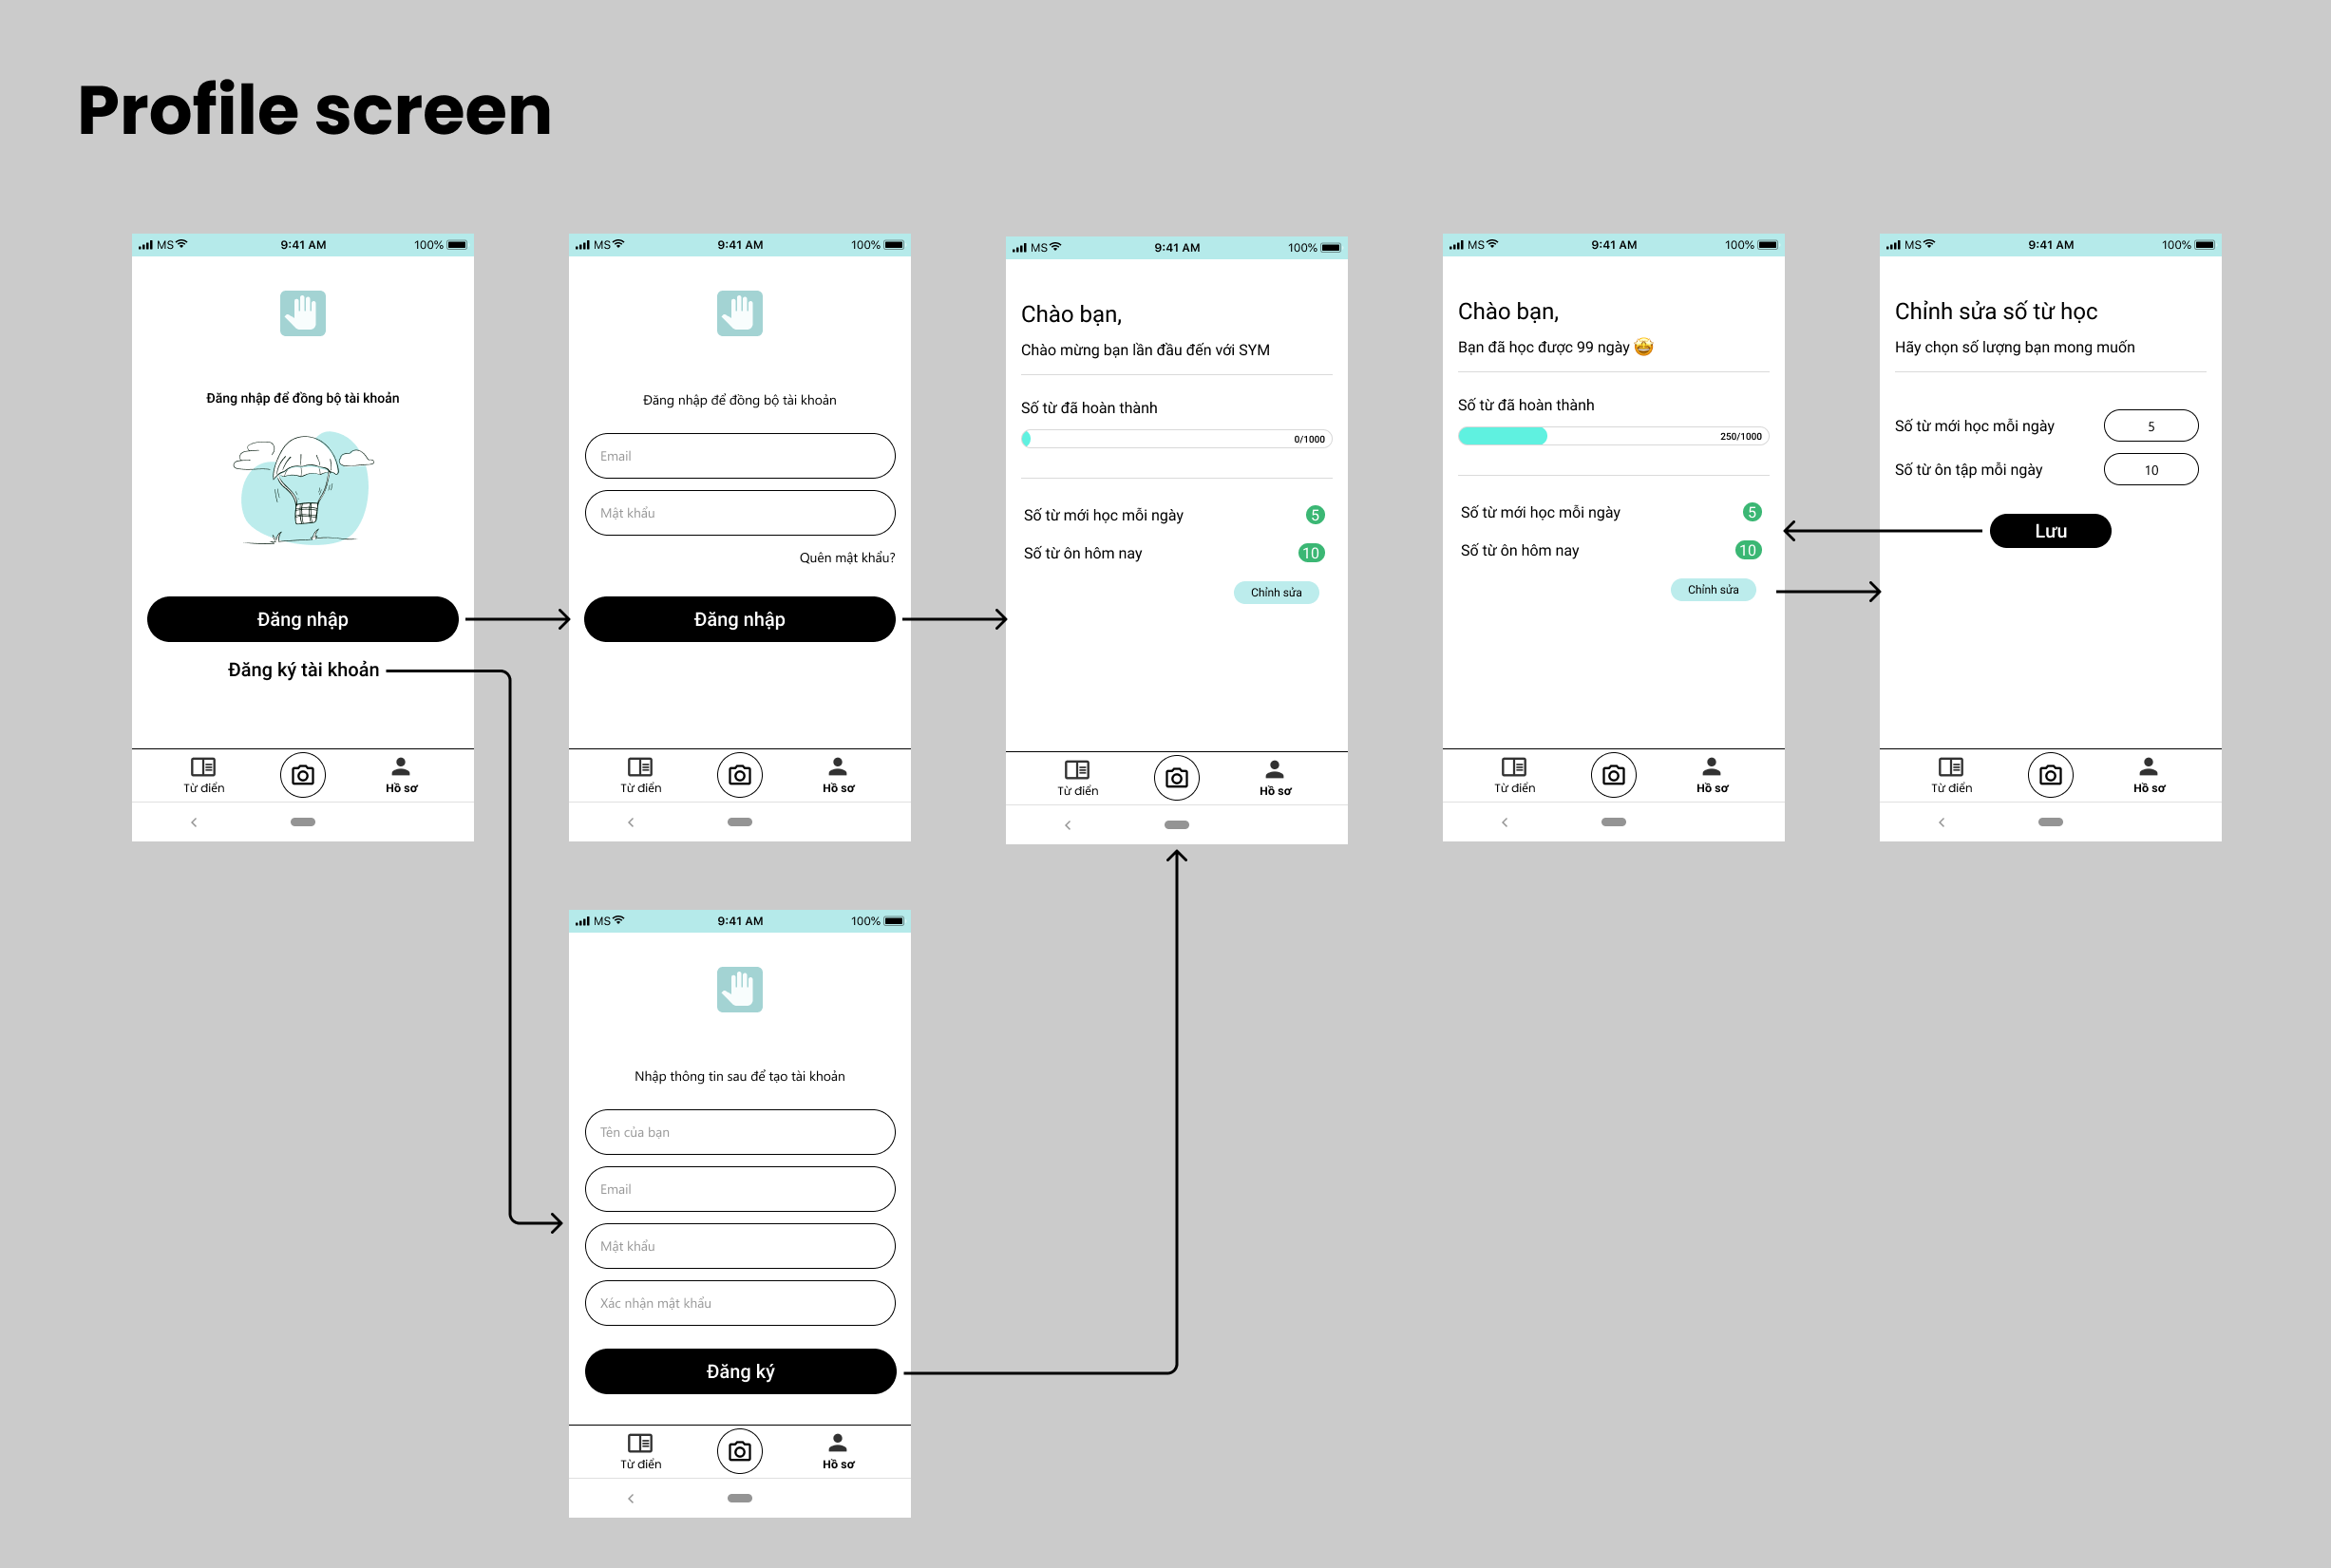
\includegraphics[width=\textwidth]{img/Chap5/Profile_screen.png}
	\caption{The main screen of the application}
\end{figure}


% Vẽ use-case
% [ ] Use-case 
%   + Xem kết quả từ được trả về sau khi dự đoán
%   + Đăng nhập/ Đăng xuất
%   + Đăng ký
%   + Xem profile
%   + Xem từ điển


% [ ] Use-case description     

\subsection{Use case}
The use case diagram is depicted in Figure \ref{fig:Chap4-usecase}

\begin{figure}[H]
	\centering
	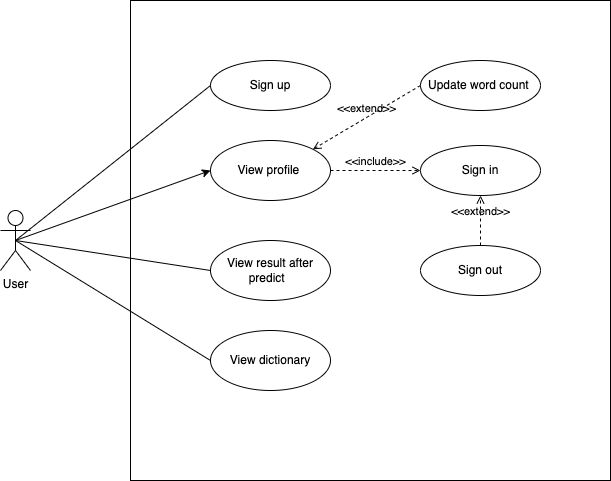
\includegraphics[width=\textwidth]{img/Chap4/use-case diagram.drawio.png}
	\caption{Use case diagram}
  \label{fig:Chap4-usecase}
\end{figure}

\subsection{Use case description}




\subsubsection{View result after predict}
\begin{table}[H]
  \centering
  \begin{tabular}{ |l| p{11cm}|}
    \hline
    Use case ID & 1 \\ 
    \hline
    Use case name & View result after predict \\ 
    \hline
        Description & The user receives information about the hand gesture he has just made\\
        \hline
        Actor & User\\
        \hline
        Post-condition(s) & Detects successful sign language and returns results to the user \\
        \hline
        \multirow{4}*{Normal flow}  & 1. User visit main page \\
        						        & 2. The user performs the operation describing the sign language\\
        					            & 3. Application that records actions and makes predictions\\
        					            & 4. The application displays the results after the prediction\\
        \hline
        \multirow{3}*{Exception flow}   & Exception1: \\
                                            & 4a. The application cannot predict the sign language\\
                                            & 5a. The application shows no more information and ends\\
        \hline
  \end{tabular}
  \caption{Use case view result after predict}
\end{table}



% Chỉnh sửa lại phần này, thêm alternative flow về việc chỉnh sửa profile
\subsubsection{View profile}
\begin{table}[H]
  \centering
  \begin{tabular}{ |l| p{11cm}|}
    \hline
    Use case ID & 2 \\ 
    \hline
    Use case name & View profile \\ 
    \hline
        Description & Users can view personal information and perform some operations to edit the number of learned words, the number of new words learned in the day.\\
        \hline
        Actor & User\\
        \hline
        Post-condition(s) & Returns the user's information \\
        \hline
        \multirow{3}*{Normal flow}  & 1. User visit profile page \\
        						        & 2. The application accesses the system to get user information\\
        					            & 3. Application that displays user information\\

        \hline
        Alternative flow & Không \\ 
        \hline
        Exception flow   & Không \\
        \hline
  \end{tabular}
  \caption{Use case view result after predict}
\end{table}


\subsubsection{Sign in}
\begin{table}[H]
  \centering
  \begin{tabular}{ |l| p{11cm}|}
    \hline
    Use case ID & 3 \\ 
    \hline
    Use case name & Sign in \\ 
    \hline
        Description & Allow users to log in to the account to use the application's services\\
        \hline
        Actor & Người dùng\\
        \hline
        Pre-condition(s) & Have an internet connection \\
        \hline
        Post-condition(s) & Logged in successfully\\
        \hline
        \multirow{4}*{Normal flow}  & 1. The application displays the login information filling interface \\
        						        & 2. User enters account name and password in 2 boxes Email, Password\\
        					            & 3. User presses "Login" button\\
                              & 4. The application shows “Logged in successfully” \\ 

        \hline
        \multirow{12}* {Alternative flow}  & A. User entered wrong login email \\
                                          & 4.1 The application shows “Error ! There is no user record
                                          corresponding to this identifier. The user may have been
                                          deleted.” \\ 
                                          & 4.2 Application goes back to step 2 \\ 
                                          & B. User enters username that is not email
                                          4.1 The application shows “Error ! The email address is badly
                                          formatted.” \\ 
                                          & 4.2 Application goes back to step 2 \\ 
                                          & C.User entered wrong password\\
                                          & 4.1 The application shows “Error ! The password is invalid.” \\ 
                                          & 4.2 Application goes back to step 2\\
        \hline
        Exception flow   & If there is no internet connection, the application displays the message "No internet connection! Please try again." \\
        \hline
  \end{tabular}
  \caption{Use case sign in}
\end{table}


\subsubsection{Sign out}
\begin{table}[H]
  \centering
  \begin{tabular}{ |l| p{11cm}|}
    \hline
    Use case ID & 4 \\ 
    \hline
    Use case name & Sign out \\ 
    \hline
        Description & Sign out\\
        \hline
        Actor & User\\
        \hline
        \multirow{2}*{Pre-condition(s)} & The device contains an application with an internet connection \\
                                        & Previously logged in \\ 
        \hline
        Post-condition(s) & Sign out successfully\\
        \hline
        \multirow{2}*{Normal flow}  & 1. The user presses the "Log Out" button \\
        						        & 2. The application returns to the login screen.\\
        \hline
        Alternative flow  & No \\
        \hline
        Exception flow   & If there is no internet connection, the application displays the message "No internet connection! Please try again." \\
        \hline
  \end{tabular}
  \caption{Use case sign out}
\end{table}



\subsubsection{Sign up}
\begin{table}[H]
  \centering
  \begin{tabular}{ |l| p{11cm}|}
    \hline
    Use case ID & 5 \\ 
    \hline
    Use case name & Sign up \\ 
    \hline
        Description & Create a personal account to be able to log into the system\\
        \hline
        Actor & User\\
        \hline
        Pre-condition(s) & Device containing the application with an internet connection \\
        \hline
        Post-condition(s) & Successful account registration\\
        \hline
        \multirow{5}*{Normal flow}  & 1. User clicks on “Create account” button \\
        						        & 2. The application displays the account registration view\\
                            & 3. The user enters the required system information \\
                            & 4. User presses “Register” button \\
                            & 5. The system returns to the login screen \\
        \hline
        \multirow{4}*{Alternative flow}   & A. The user stopped creating an account and wants to go back to the login screen \\
                                          & User presses “Login here” button and the application jumps to step 5 \\
        \hline
        Exception flow   & If there is no internet connection, the application displays the message "No internet connection! Please try again." \\
        \hline
  \end{tabular}
  \caption{Use case sign up}
\end{table}